\documentclass{standalone}
\usepackage{tikz}
\usetikzlibrary{patterns, positioning}

\begin{document}
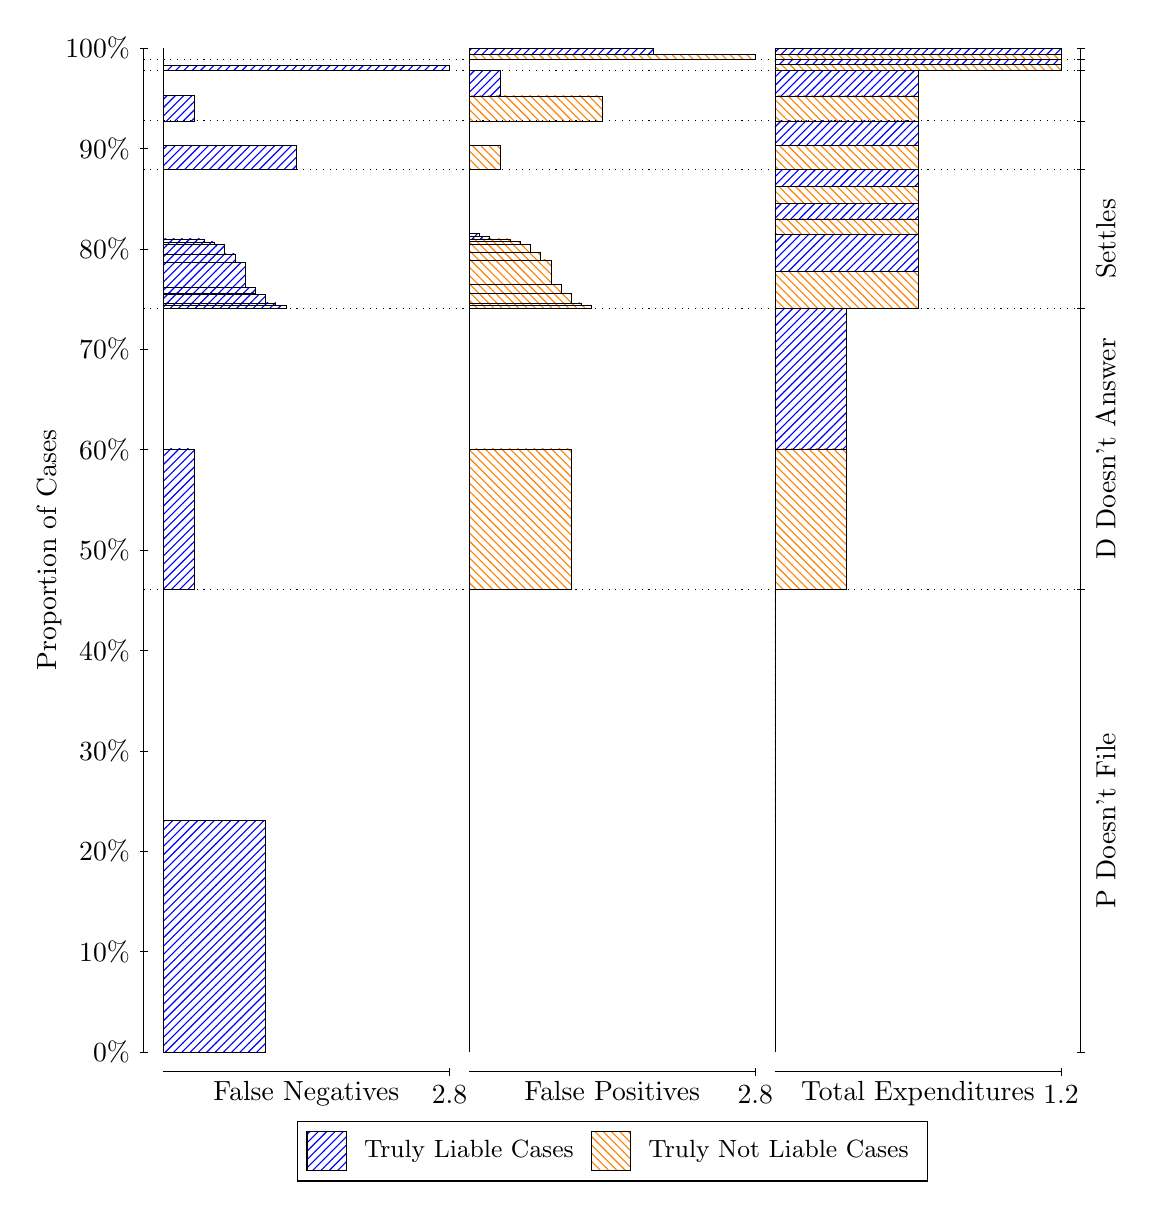
\begin{tikzpicture}
\draw[black, very thin] (1.5,1.75) -- (1.5,14.5);
\node[rotate=90, anchor=center] at (0.3, 8.125) {Proportion of Cases};
\draw[black, very thin] (1.45,1.75) -- (1.55,1.75);
\node[anchor=east] at (1.45, 1.75) {0\%};
\draw[black, very thin] (1.45,3.025) -- (1.55,3.025);
\node[anchor=east] at (1.45, 3.025) {10\%};
\draw[black, very thin] (1.45,4.3) -- (1.55,4.3);
\node[anchor=east] at (1.45, 4.3) {20\%};
\draw[black, very thin] (1.45,5.575) -- (1.55,5.575);
\node[anchor=east] at (1.45, 5.575) {30\%};
\draw[black, very thin] (1.45,6.85) -- (1.55,6.85);
\node[anchor=east] at (1.45, 6.85) {40\%};
\draw[black, very thin] (1.45,8.125) -- (1.55,8.125);
\node[anchor=east] at (1.45, 8.125) {50\%};
\draw[black, very thin] (1.45,9.4) -- (1.55,9.4);
\node[anchor=east] at (1.45, 9.4) {60\%};
\draw[black, very thin] (1.45,10.675) -- (1.55,10.675);
\node[anchor=east] at (1.45, 10.675) {70\%};
\draw[black, very thin] (1.45,11.95) -- (1.55,11.95);
\node[anchor=east] at (1.45, 11.95) {80\%};
\draw[black, very thin] (1.45,13.225) -- (1.55,13.225);
\node[anchor=east] at (1.45, 13.225) {90\%};
\draw[black, very thin] (1.45,14.5) -- (1.55,14.5);
\node[anchor=east] at (1.45, 14.5) {100\%};

\draw[black, very thin] (13.4,1.75) -- (13.4,14.5);
\draw[black, very thin] (13.35,1.75) -- (13.45,1.75);
\node[anchor=west] at (13.35, 1.75) {};
\draw[black, very thin] (13.35,7.6226) -- (13.45,7.6226);
\node[anchor=west] at (13.35, 7.6226) {};
\draw[black, very thin] (13.35,11.193) -- (13.45,11.193);
\node[anchor=west] at (13.35, 11.193) {};
\draw[black, very thin] (13.35,12.958) -- (13.45,12.958);
\node[anchor=west] at (13.35, 12.958) {};
\draw[black, very thin] (13.35,13.575) -- (13.45,13.575);
\node[anchor=west] at (13.35, 13.575) {};
\draw[black, very thin] (13.35,14.213) -- (13.45,14.213);
\node[anchor=west] at (13.35, 14.213) {};
\draw[black, very thin] (13.35,14.357) -- (13.45,14.357);
\node[anchor=west] at (13.35, 14.357) {};
\draw[black, very thin] (13.35,14.5) -- (13.45,14.5);
\node[anchor=west] at (13.35, 14.5) {};

\draw[black, very thin, pattern color=blue, pattern=north east lines] (1.75,1.75) rectangle (3.0476,4.6863);
\draw[black, very thin, pattern color=orange, pattern=north west lines] (1.75,4.6863) rectangle (1.75,7.6226);
\draw[black, very thin, pattern color=blue, pattern=north east lines] (1.75,7.6226) rectangle (2.1393,9.408);
\draw[black, very thin, pattern color=orange, pattern=north west lines] (1.75,9.408) rectangle (1.75,11.193);
\draw[black, very thin, pattern color=blue, pattern=north east lines] (1.75,11.193) rectangle (3.3071,11.228);
\draw[black, very thin, pattern color=blue, pattern=north east lines] (1.75,11.228) rectangle (3.1774,11.262);
\draw[black, very thin, pattern color=blue, pattern=north east lines] (1.75,11.262) rectangle (3.0476,11.367);
\draw[black, very thin, pattern color=blue, pattern=north east lines] (1.75,11.367) rectangle (2.9179,11.39);
\draw[black, very thin, pattern color=blue, pattern=north east lines] (1.75,11.39) rectangle (2.9179,11.46);
\draw[black, very thin, pattern color=blue, pattern=north east lines] (1.75,11.46) rectangle (2.7881,11.776);
\draw[black, very thin, pattern color=blue, pattern=north east lines] (1.75,11.776) rectangle (2.6583,11.885);
\draw[black, very thin, pattern color=blue, pattern=north east lines] (1.75,11.885) rectangle (2.5286,12.005);
\draw[black, very thin, pattern color=blue, pattern=north east lines] (1.75,12.005) rectangle (2.3988,12.039);
\draw[black, very thin, pattern color=blue, pattern=north east lines] (1.75,12.039) rectangle (2.269,12.076);
\draw[black, very thin, pattern color=orange, pattern=north west lines] (1.75,12.076) rectangle (1.75,12.958);
\draw[black, very thin, pattern color=blue, pattern=north east lines] (1.75,12.958) rectangle (3.4369,13.265);
\draw[black, very thin, pattern color=orange, pattern=north west lines] (1.75,13.265) rectangle (1.75,13.575);
\draw[black, very thin, pattern color=blue, pattern=north east lines] (1.75,13.575) rectangle (2.1393,13.896);
\draw[black, very thin, pattern color=orange, pattern=north west lines] (1.75,13.896) rectangle (1.75,14.213);
\draw[black, very thin, pattern color=blue, pattern=north east lines] (1.75,14.213) rectangle (5.3833,14.279);
\draw[black, very thin, pattern color=orange, pattern=north west lines] (1.75,14.279) rectangle (1.75,14.357);
\draw[black, very thin, pattern color=orange, pattern=north west lines] (1.75,14.357) rectangle (1.75,14.423);
\draw[black, very thin, pattern color=blue, pattern=north east lines] (1.75,14.423) rectangle (1.75,14.5);
\draw[black, very thin, pattern color=orange, pattern=north west lines] (5.6333,1.75) rectangle (5.6333,4.6863);
\draw[black, very thin, pattern color=blue, pattern=north east lines] (5.6333,4.6863) rectangle (5.6333,7.6226);
\draw[black, very thin, pattern color=orange, pattern=north west lines] (5.6333,7.6226) rectangle (6.931,9.408);
\draw[black, very thin, pattern color=blue, pattern=north east lines] (5.6333,9.408) rectangle (5.6333,11.193);
\draw[black, very thin, pattern color=orange, pattern=north west lines] (5.6333,11.193) rectangle (7.1905,11.23);
\draw[black, very thin, pattern color=orange, pattern=north west lines] (5.6333,11.23) rectangle (7.0607,11.264);
\draw[black, very thin, pattern color=orange, pattern=north west lines] (5.6333,11.264) rectangle (6.931,11.385);
\draw[black, very thin, pattern color=orange, pattern=north west lines] (5.6333,11.385) rectangle (6.8012,11.494);
\draw[black, very thin, pattern color=orange, pattern=north west lines] (5.6333,11.494) rectangle (6.6714,11.81);
\draw[black, very thin, pattern color=orange, pattern=north west lines] (5.6333,11.81) rectangle (6.5417,11.902);
\draw[black, very thin, pattern color=orange, pattern=north west lines] (5.6333,11.902) rectangle (6.4119,12.006);
\draw[black, very thin, pattern color=orange, pattern=north west lines] (5.6333,12.006) rectangle (6.2821,12.041);
\draw[black, very thin, pattern color=orange, pattern=north west lines] (5.6333,12.041) rectangle (6.1524,12.075);
\draw[black, very thin, pattern color=blue, pattern=north east lines] (5.6333,12.075) rectangle (5.8929,12.112);
\draw[black, very thin, pattern color=blue, pattern=north east lines] (5.6333,12.112) rectangle (5.7631,12.146);
\draw[black, very thin, pattern color=blue, pattern=north east lines] (5.6333,12.146) rectangle (5.6333,12.958);
\draw[black, very thin, pattern color=orange, pattern=north west lines] (5.6333,12.958) rectangle (6.0226,13.268);
\draw[black, very thin, pattern color=blue, pattern=north east lines] (5.6333,13.268) rectangle (5.6333,13.575);
\draw[black, very thin, pattern color=orange, pattern=north west lines] (5.6333,13.575) rectangle (7.3202,13.893);
\draw[black, very thin, pattern color=blue, pattern=north east lines] (5.6333,13.893) rectangle (6.0226,14.213);
\draw[black, very thin, pattern color=orange, pattern=north west lines] (5.6333,14.213) rectangle (5.6333,14.291);
\draw[black, very thin, pattern color=blue, pattern=north east lines] (5.6333,14.291) rectangle (5.6333,14.357);
\draw[black, very thin, pattern color=orange, pattern=north west lines] (5.6333,14.357) rectangle (9.2667,14.423);
\draw[black, very thin, pattern color=blue, pattern=north east lines] (5.6333,14.423) rectangle (7.969,14.5);
\draw[black, very thin, pattern color=orange, pattern=north west lines] (9.5167,1.75) rectangle (9.5167,4.6863);
\draw[black, very thin, pattern color=blue, pattern=north east lines] (9.5167,4.6863) rectangle (9.5167,7.6226);
\draw[black, very thin, pattern color=orange, pattern=north west lines] (9.5167,7.6226) rectangle (10.425,9.408);
\draw[black, very thin, pattern color=blue, pattern=north east lines] (9.5167,9.408) rectangle (10.425,11.193);
\draw[black, very thin, pattern color=orange, pattern=north west lines] (9.5167,11.193) rectangle (11.333,11.664);
\draw[black, very thin, pattern color=blue, pattern=north east lines] (9.5167,11.664) rectangle (11.333,12.134);
\draw[black, very thin, pattern color=orange, pattern=north west lines] (9.5167,12.134) rectangle (11.333,12.329);
\draw[black, very thin, pattern color=blue, pattern=north east lines] (9.5167,12.329) rectangle (11.333,12.526);
\draw[black, very thin, pattern color=orange, pattern=north west lines] (9.5167,12.526) rectangle (11.333,12.741);
\draw[black, very thin, pattern color=blue, pattern=north east lines] (9.5167,12.741) rectangle (11.333,12.958);
\draw[black, very thin, pattern color=orange, pattern=north west lines] (9.5167,12.958) rectangle (11.333,13.268);
\draw[black, very thin, pattern color=blue, pattern=north east lines] (9.5167,13.268) rectangle (11.333,13.575);
\draw[black, very thin, pattern color=orange, pattern=north west lines] (9.5167,13.575) rectangle (11.333,13.893);
\draw[black, very thin, pattern color=blue, pattern=north east lines] (9.5167,13.893) rectangle (11.333,14.213);
\draw[black, very thin, pattern color=orange, pattern=north west lines] (9.5167,14.213) rectangle (13.15,14.291);
\draw[black, very thin, pattern color=blue, pattern=north east lines] (9.5167,14.291) rectangle (13.15,14.357);
\draw[black, very thin, pattern color=orange, pattern=north west lines] (9.5167,14.357) rectangle (13.15,14.423);
\draw[black, very thin, pattern color=blue, pattern=north east lines] (9.5167,14.423) rectangle (13.15,14.5);
\draw[black, dotted] (1.5,7.6226) -- (13.4,7.6226);
\draw[black, dotted] (1.5,11.193) -- (13.4,11.193);
\draw[black, dotted] (1.5,12.958) -- (13.4,12.958);
\draw[black, dotted] (1.5,13.575) -- (13.4,13.575);
\draw[black, dotted] (1.5,14.213) -- (13.4,14.213);
\draw[black, dotted] (1.5,14.357) -- (13.4,14.357);
\draw[black, very thin] (1.75,1.5) -- (5.3833,1.5);
\node[anchor=north] at (3.5667, 1.5) {False Negatives};
\draw[black, very thin] (5.3833,1.45) -- (5.3833,1.55);
\node[anchor=north] at (5.3833, 1.45) {2.8};

\draw[black, very thin] (5.6333,1.5) -- (9.2667,1.5);
\node[anchor=north] at (7.45, 1.5) {False Positives};
\draw[black, very thin] (9.2667,1.45) -- (9.2667,1.55);
\node[anchor=north] at (9.2667, 1.45) {2.8};

\draw[black, very thin] (9.5167,1.5) -- (13.15,1.5);
\node[anchor=north] at (11.333, 1.5) {Total Expenditures};
\draw[black, very thin] (13.15,1.45) -- (13.15,1.55);
\node[anchor=north] at (13.15, 1.45) {1.2};

\node[black, centered, rotate=90] at (13.72, 4.6863) {P Doesn't File};
\node[black, centered, rotate=90] at (13.72, 9.408) {D Doesn't Answer};
\node[black, centered, rotate=90] at (13.72, 12.076) {Settles};





\draw (7.449999999999999,1.5) node[draw=none] (baseCoordinate) {};
\begin{scope}[align=center]
        \matrix[scale=0.5, draw=black, below=0.5cm of baseCoordinate, nodes={draw}, column sep=0.1cm]{
            \node[rectangle, draw, minimum width=0.5cm, minimum height=0.5cm, pattern=north east lines, pattern color=blue] {}; &
            \node[draw=none, font=\small] (B) {Truly Liable Cases}; &
            \node[rectangle, draw, minimum width=0.5cm, minimum height=0.5cm, pattern=north west lines, pattern color=orange] {}; &
            \node[draw=none, font=\small] (B) {Truly Not Liable Cases}; \\
            };
\end{scope}

\end{tikzpicture}
\end{document}